 % -----------------------------------------------
% Template for SMC 2009
%     smc2009.sty -> style file
% Last modified by Fabien Gouyon (smc2009@inescporto.pt)
% Modified by Juan P. Bello (ismir2008-papers@ismir.net)
% By Rainer Typke (ismir07.rainer@safersignup.com)
% Based on the 2004 template by Eloi Batlle.
% -----------------------------------------------

\documentclass{article}
\usepackage{stsm2009,amsmath}
% To use when using pdflatex
\usepackage{graphicx}
\usepackage{url}     
\usepackage{hyperref}  
      
\newenvironment{packed_item}{
\begin{itemize}
  \setlength{\itemsep}{1pt}
  \setlength{\parskip}{0pt}
  \setlength{\parsep}{0pt}
}{\end{itemize}}

\newenvironment{packed_enumerate}{
\begin{enumerate}
  \setlength{\itemsep}{1pt}
  \setlength{\parskip}{0pt}
  \setlength{\parsep}{0pt}
}{\end{enumerate}}
% To use when using latex, dvips and ps2pdf
% \usepackage[dvips]{graphicx}


\title{ADVANCED REAL-TIME CONTROL OF PARAMETERS \\BY INTEGRATION OF JAMOMA AND FTM IN MAX.\\
Report of a COST IC0601 SID Short-Term Scientific Mission April 2009 \\Hosted by The Real-Time Musical Interactions Team, IRCAM, Paris (FR)}
% IMPORTANT NOTICE:
% Reviews are double-blind
% Authors will not be informed of who reviews their papers, and author names will be concealed from the reviewers 
% Please avoid evident self references in the text

% Authors' names must be omitted from title page (or listed as Òname(s) omitted for submissionÓ)


% Single address
% To use with only one author or several with the same address
% ---------------
\oneauthor
   {Trond Lossius} {BEK - Bergen Center for Electronic Arts \\ Bergen (NO) \\ trond.lossius@bek.no} 
 


% Two addresses
 %--------------
%\threeauthors
%  {First author} {School \\ Email}
%  {Second author} {Company \\ Email}
%  {Third author} {Company \\ Email}
% Three addresses
% --------------
%\threeauthors
%  {First author} {School \\ Email}
%  {Second author} {Company \\ Email}
%  {Third author} {Company \\ Email}

\begin{document}
%    
\sloppy
\maketitle
%

\permission

\begin{abstract}  



\end{abstract}

\section{Introduction}\label{sec:introduction}        


\subsection{Real-time technologies in the arts.}\label{sec:intro-real-time}

The development of real-time technology has opened new possibilities for artistic expression, enabling live generation of and interaction with media. The processing in real-time of media and live input, often combined with possibilities for physical computing \cite{Sullivan_2004_physical_computing}, has become an integrated part of a variety of contemporary artistic practises such as works for stage, live music performances using New Instruments for Musical Expression, interactive and generative installations and sound art. A major challenge in this kind of works is how to develop control systems that maintain access to a rich set of parameters while remaining manageable in a live performance setting.

\subsection{Jamoma: Accessing complex sets of parameters in real-time through a structured approach.}\label{sec:intro-accessing}

Max/MSP/Jitter is one of several programming environments for real time processing of media. According to one of its creators ``Max/MSP does not enforce readability, consistency, or efficiency on its users. There are no real standards for interoperability at the level of the patcher.'' \cite{Zicarelli:2002_program_that_do_nothing}.

Jamoma attempts to address this issue by providing a framework for modular development in Max with a structured API for interfacing with modules \cite{Place:2006jamoma}. Jamoma modules communicate using the Open Sound Control (OSC) protocol \cite{Wright_2002_OSC}, extended through an object-oriented approach to OSC nodes, conceiving them as having properties and methods \cite{Place:2008osc_properties}. The process of assigning additional properties to parameters defining their behaviour increase the abilities for continuous transformation and shaping of the artistic material \cite{Place_2008_flexible_control}. The OSC namespace implementation in Jamoma also provides possibilities of querying the system for the namespace of available nodes, as well as retrieving information on current values of nodes and node properties, along somewhat similar lines as suggested by \cite{Jazzmutant:2006_osc2}. This way Jamoma partly offers solutions to a fundamental question of how to maintain access to and control of complex sets of parameters and data in real-time systems.

Apart from being used for artistic purposes, Jamoma is also used for research and prototyping of protocols for capturing and communication of data streams, e.g. gestural data using GDIF - Gestural Description Interchange Format \cite{Jensenius:2006a, Nymoen_2008_GDIF_sync} and spatial audio information according to SpatDIF - Spatial Sound Description Interchange Format (Peters, 2008).

\subsection{Controlling complex sets of parameters in real-time environments.}\label{sec:intro-complex-control}

The Jamoma  API offers simple access to all parameters of all modules, but relatively few modules so far takes advantage of this for advanced controlling purposes. The main exceptions are two modules providing text-based cue list systems, a number of modules for one-to-one mappings between parameter values, and a series of modules for work on SDIF - Sound Description Interchange Format data \cite{Nymoen_2008_GDIF_sync}. In addition \emph{Virage Sequencer} is currently being development within the framework the Virage Platform as a stand-alone OSC sequencer able to interface with Jamoma \footnote{http://www.plateforme-virage.org/}.

FTM is a shared library and a set of modules extending the signal and message data flow paradigm of Max permitting the representation and processing of complex data structures such as matrices, sequences or dictionaries as well as tuples, MIDI events or score elements \cite{Schnell:2005ftm}. FTM forms the basis for the MnM toolbox, dedicated to mapping between gesture and sound, and more generally to statistical and machine learning methods \cite{Bevilacqua:2005mnm}, as well as Gabor, a unified framework for a number of advanced audio processing techniques \cite{Schnell_2005_Gabor}.




%%%%%%%%%%%%%%%%%%%%%%%%%%%%%%%%%%%%%%%%%%%%%%%%%%%%%%%%%%%%%%%%%%%%%%%%%%%%%
%
%%%%%%%%%%%%%%%%%%%%%%%%%%%%%%%%%%%%%%%%%%%%%%%%%%%%%%%%%%%%%%%%%%%%%%%%%%%%%

\section{Querying OSC namespace and node properties in Jamoma.}  
 
\begin{figure*}[!t] \centerline{
		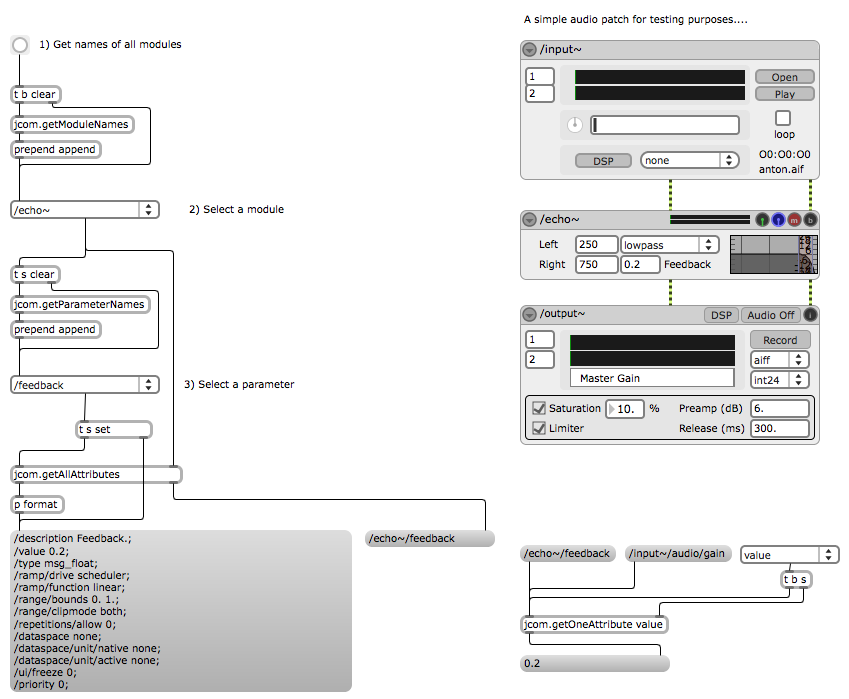
\includegraphics[width=1.8\columnwidth]{SID-STSM-jamomaQuery.png}} \caption{Example patch illustrating the process of querying Jamoma modules for OSC namespace and node properties.} \label{fig:querying} 
	\end{figure*}

Mechanisms for querying Jamoma modules for their nodes and properties are implemented as part of the Jamoma Core C++ externals for Max utilised in all modules. A number of \emph{components} or Max abstractions made to behave like externals have been developed to simplify the process of performing queries:

\begin{itemize}
	
	\item \emph{jcom.getModules} when banged will dump the OSC names of all module instances that are currently running on the client.

	\item The OSC addresses of parameters, messages and returns of a module can be queried by passing the OSC name of a module to the components \emph{jcom.getParameterNames} \emph{jcom.getMessageNames} and \emph{jcom.getReturnNames} respectively. \footnote{\emph{Parameters} are OSC nodes stored as part of the state of the module. \emph{Messages} behave the same as parameters, except that they are stateless. \emph{Returns} are used when the module algorithm generate new data returned as OSC messages, but this data is not stored as part of the state of the module itself.}

	\item Parameters, messages and returns in Jamoma are enhanced by the addition of properties and methods, controlling the data type, range, ramps to new values, filtering of repetitions etc. \cite{Place:2006jamoma, Place:2008osc_properties, Place_2008_flexible_control}. By passing the OSC name of a module and a node (parameter, message or return) of that module to the component \emph{jcom.getAllAttributes}, current values of all properties of that node will be returned, including the value of the node itself. The component \emph{jcom.getOneAttribute} can be used to query the property of one attribute only.
		
\end{itemize}

Figure \ref{fig:querying} illustrates the use of these components to investigate a simple patch containing three Jamoma modules.

In addition to instant queries of current state of Jamoma modules, the externals \emph{jcom.send} and \emph{jcom.receive} can be used to tap into live streams of OSC data passing through Jamoma. This will on an ongoing basis catch changes to all parameters of all modules as well as any returned OSC messages generated internally by Jamoma modules.

As an addition to the online documentation of Jamoma, a tutorial has been added on how to retrieve information about existing Jamoma modules \footnote{http://groupware.bek.no/groups/jamoma/wiki/f11fc/ \\ Retrieving\_information\_about\_existing\_Jamoma\_modules.html}.


%%%%%%%%%%%%%%%%%%%%%%%%%%%%%%%%%%%%%%%%%%%%%%%%%%%%%%%%%%%%%%%%%%%%%%%%%%%%%
%
%%%%%%%%%%%%%%%%%%%%%%%%%%%%%%%%%%%%%%%%%%%%%%%%%%%%%%%%%%%%%%%%%%%%%%%%%%%%%

\section{Storing properties in FTM.}

\subsection{Storing information on the namespace as a matrix.}

\subsection{Recording events as sequences.}

\subsection{Compound data}


%%%%%%%%%%%%%%%%%%%%%%%%%%%%%%%%%%%%%%%%%%%%%%%%%%%%%%%%%%%%%%%%%%%%%%%%%%%%%
%
%%%%%%%%%%%%%%%%%%%%%%%%%%%%%%%%%%%%%%%%%%%%%%%%%%%%%%%%%%%%%%%%%%%%%%%%%%%%%

\section{Controlling Jamoma by manipulation of FTM data objects.}

\subsection{Test patches.}

\subsubsection{Modulus interacting with physical devices.}


\subsubsection{Modules for audio processing}




%%%%%%%%%%%%%%%%%%%%%%%%%%%%%%%%%%%%%%%%%%%%%%%%%%%%%%%%%%%%%%%%%%%%%%%%%%%%%
%
%%%%%%%%%%%%%%%%%%%%%%%%%%%%%%%%%%%%%%%%%%%%%%%%%%%%%%%%%%%%%%%%%%%%%%%%%%%%%

\section{Discussion \& Conclusion.}


\subsection{Towards a layered model for control of real-time systems}



%%%%%%%%%%%%%%%%%%%%%%%%%%%%%%%%%%%%%%%%%%%%%%%%%%%%%%%%%%%%%%%%%%%%%%%%%%%%%
%
%%%%%%%%%%%%%%%%%%%%%%%%%%%%%%%%%%%%%%%%%%%%%%%%%%%%%%%%%%%%%%%%%%%%%%%%%%%%%

\section{Acknowledgment.}

 The COST IC0601 Action on Sonic Interaction Design (SID) .


\bibliographystyle{abbrv}  %\bibliographystyle{natbib}% ama, nar, alpha, plain, chicago,{plainnat}  abbrv, siam   
\small
\bibliography{stsm09}
\end{document}   



% \section{Style Stuff - delme}

% \subsection{Title and Authors}

%The title is 14pt Times, bold, caps, upper case, centered. Authors' names are centered. 
%The lead author's name is to be listed first (left-most), and the co-authors' names after. If the addresses for all 
%authors are the same, include the address only once, centered. If the authors have different addresses, 
%put the addresses, evenly spaced, under each authors' name.

% Reviews are double-blind. {\it \textbf{Author information should be removed from this page in initial submissions}}, 
% and only added later by the authors when sending camera-ready versions.

%\subsection{Figures, Tables and Captions}

%All artwork must be centered, neat, clean, and legible. All lines should
%be very dark for purposes of reproduction and art work should not be hand-drawn.
%The proceedings is not in color, and therefore all figures must make
%sense in black-and-white form.
%Figure and table numbers and captions always appear below the figure. Leave 1
%line space between the figure or table and the caption. Each figure or table
%is numbered consecutively. Captions should be Times 10pt.
%Place tables/figures in text as close to the reference as possible.
%References to figures and tables should be capitalised, for example:
%see Figure \ref{fig:example} and Table \ref{tab:example}.
%Figures and tables may extend across both columns to a maximum
%width of 7'' (17.78~cm).

%\begin{table}
%\begin{center}
%\begin{tabular}{|l|l|}
%\hline
%String value & Numeric value \\
%\hline
%hello SMC  & 1073 \\
%\hline
%\end{tabular}
%\end{center}
%\caption{Table captions should be placed below the table}
%\label{tab:example}
%\end{table}

%\begin{figure}
%\centerline{\framebox{
% To use when using pdflatex
%	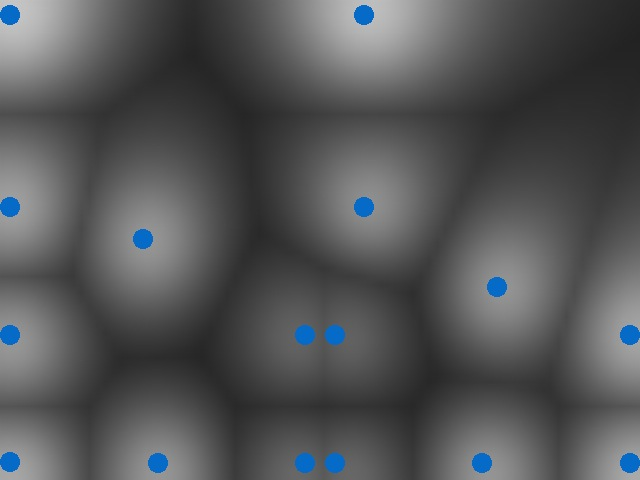
\includegraphics[width=\columnwidth]{../ICMC2009-dbap/all_r_6_b_0_2}}}
	% To use when using latex, dvips and ps2pdf
% 	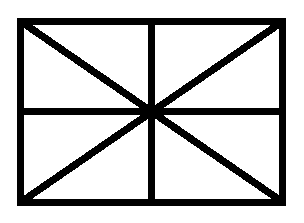
\includegraphics[width=\columnwidth]{figure.eps}}}
%\caption{Figure captions should be placed below the figure}
%\label{fig:example}
%\end{figure}